%
% main.tex -- Paper zum Thema fpga
%
% (c) 2019 Hochschule Rapperswil
%

\graphicspath{papers/fpga/}

\chapter{VHDL Implementation of the Fast Wavelet Transform\label{chapter:fpga}}
\lhead{VHDL Implementation of the Fast Wavelet Transform}
\begin{refsection}
\chapterauthor{Jonas Gründler and Nicolas Tobler}

\section{Introduction}
\rhead{Introduction}

VHDL, an acronym for Very High Speed Integrated Circuit Hardware Description Language, is commonly used to implement fast, application-specific logic for an FPGA or custom silicon chip.
As every other programming language, VHDL relies heavily on reuse of code.
Blocks of encapsulated code can be stored as a semiconductor intellectual property core (IP core) and reused for further applications.
A often used IP core is the Fast Fourier Transform (FFT), which is available online for free.
Discrete wavelet transforms (DWT), however, are not that common.
Therefore, we have committed ourselfs to implementing a wavelet transform as a hardware block in VHDL.

A hardware implementation of a wavelet transform has many advantages over a software implementation.
First, chained arithmetic operations in hardware can be executed much faster than in software.
A CPU, in contrast, is bound to a limited instruction set and needs multiple clock cycles for the same operation.
Some of the operations can be executed in parallel to gain even more speed.
Secondly, if stream based processing is implemented, which continuously processes incoming data, the latency can be significantly lowered.
This property makes hardware superior for real time applications.

In the first part, this work covers the theory of an efficient algorithm for the discrete wavelet transform.
Then, an implementation of this algorithm in VHDL is presented.

\section{Discrete Wavelet Transform}
\rhead{Discrete Wavelet Transform}

The DTW is covered in detail in chapter \ref{section:schnelle-synthese} of part 1.
This section provides a short summary, as well as some additions, notably the lifting scheme.

The discrete wavelet transform is defined by a pair of formulas to calculate the wavelet coefficients $\bm a$ and $\bm b$.
$a_{j,k}$ and $b_{j,k}$ represent the coefficients in layer $j$ at the discrete time step $k$.
The formula to calculate the forward DWT is
\begin{align}
a_{j,k} &= \sum_{l} \bar{h}_l a_{j+1,l+2k}
\\
b_{j,k} &= \sum_{l} \bar{g}_l a_{j+1,l+2k} .
\end{align}
This calculation uses the father and mother wavelet coefficients $\bm{\bar h}$ and $\bm{\bar g}$, which are given by the chosen wavelet.
The inverse transform has been derived in the part 1 as well: 
\begin{align}
a_{j+1,k} =
\sum_{l\in\mathbb Z}
h_{k-2l}
a_{j,l}
+
\sum_{l\in\mathbb Z}
g_{k-2l}
b_{j,l} .
\end{align}
In order to create a connection between the theory covered in the script and additional theory, the $z$-transform is used.
The $z$-transform of a FIR (finite impulse response) filter $h$ is a Laurent polynomial given by
\begin{equation}
h(z) = \sum_{k} h_k z^{-k}
\end{equation}
A convolution is equal to a multiplication in the $z$-domain.
Thus, the formulas from part 1 can be rewritten in the $z$-transform notation.
The forward transform becomes
\begin{align}
\quad a_{j,k}(z) &= \bar h(z^{-1}) a_{j+1,2k}(z) 
\\
\quad b_{j,k}(z) &= \bar g(z^{-1}) a_{j+1,2k}(z),
\end{align}
while the backward transform is
\begin{equation}
a_{j+1,k}(z) = h(z) a_{j,k}(z) + g(z) b_{j,k}(z).
\end{equation}
Figure \ref{fpga:fig:dwt} depicts the computational flow graph of the DWT followed by an inverse DWT.
\begin{figure}
	\centering
	\usetikzlibrary{automata,arrows,positioning,calc}


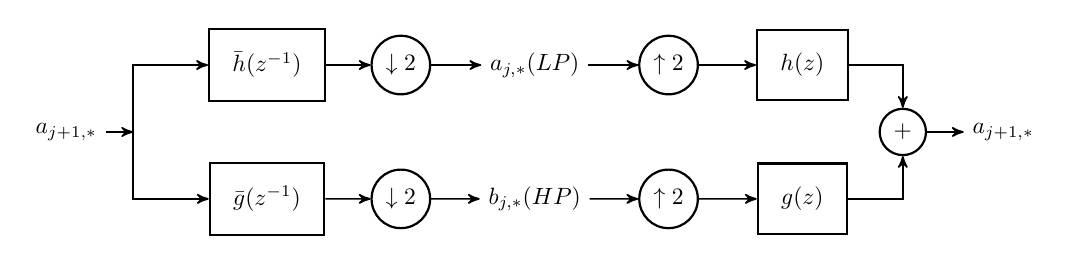
\begin{tikzpicture}[->, >=stealth', auto, semithick, node distance=2cm, scale = 0.85]

%\useasboundingbox (0,-0.5) rectangle (12.5,1.5);

\tikzstyle{every state}=[fill=white,draw=black,thick,text=black, scale = 1]
\tikzstyle{block}=[rectangle, inner sep=10pt, fill=white,draw=black,thick,text=black, scale = 1]
\tikzstyle{square}=[rectangle, fill=white,draw=black,thick,text=black, minimum height = 0.8cm, minimum width = 0.8cm, scale = 1]
\tikzstyle{round}=[circle, fill=white,draw=black,thick,text=black, scale = 1]
\tikzstyle{dots}=[fill=white,thick,text=black,scale=1]

\tikzset{every node/.style={scale=0.85}}
\tikzset{every coordinate/.style={scale=0.85}}

%\draw[step=1.0,black,thin,xshift=0.0cm,yshift=0.0cm] (-1,-3) grid (15,3);

\node[dots] (start) at (0,0) {$a_{j+1,*}$};

\coordinate     (split) at (1,0);

\node[block] (h1) at (3,1) {$\bar h(z^{-1})$};
\node[block] (h2) at (3,-1) {$\bar g(z^{-1})$};

\node[round] (d1) [right of=h1] {$\downarrow 2$};
\node[round] (d2) [right of=h2] {$\downarrow 2$};

\node[dots] (dots1) [right of=d1] {$a_{j,*} \- \text{(LP)}$};
\node[dots] (dots2) [right of=d2] {$b_{j,*} \- \text{(HP)}$};

\node[round] (u1) [right of=dots1] {$\uparrow 2$};
\node[round] (u2) [right of=dots2] {$\uparrow 2$};

\node[block] (hh1) [right of=u1] {$ h(z)$};
\node[block] (hh2) [right of=u2] {$ g(z)$};

\node[round] (combine) at (12.5,0) {$+$};

\node[dots, right of=combine, node distance=1.5cm] (end) {$a_{j+1,*}$} ;

\draw[->] (start) -- node {}(split);

\draw[->] (split) |- node {}(h1);
\draw[->] (split) |- node {}(h2);

\draw[->] (h1) -- node {}(d1);
\draw[->] (h2) -- node {}(d2);

\draw[->] (d1) -- node {}(dots1);
\draw[->] (d2) -- node {}(dots2);

\draw[->] (dots1) -- node {}(u1);
\draw[->] (dots2) -- node {}(u2);

\draw[->] (u1) -- node {}(hh1);
\draw[->] (u2) -- node {}(hh2);

\draw[->] (hh1) -| node {}(combine);
\draw[->] (hh2) -| node {}(combine);

\draw[->] (combine) -- node {}(end);

\end{tikzpicture}
	\caption{Discrete Wavelet transform and inverse transform}
	\label{fpga:fig:dwt}
\end{figure}
The DWT splits an input signal into only two wavelet coefficients.
If more details are required, a multiresolution analysis can be performed.
An input signal $\bm x$, where $x_k$ is its value at time step $k$, can be transformed into a tower of wavelet coefficients.
$x_t$ is set equal to $a_{0,k}$ and represents the first layer of the tower.
The $a_{i,k}$ coefficients are now recursively transformed into $a_{i-1,k}$ and $b_{i-1,k}$ coefficients
This tower can be arbitrarily long and leads to a bigger frequency range.
From all generated coefficients, only $\bm b$ and the last layer of $\bm a$ coefficients are required since they hold all information needed for a reconstuction of the input signal.
Figure \ref{fpga:fig:dwtTower} shows a decomposition of 3 levels using DWTs and a subsequent unification using inverse DWTs.
\begin{figure}
	\centering
	\usetikzlibrary{automata,arrows,positioning,calc}

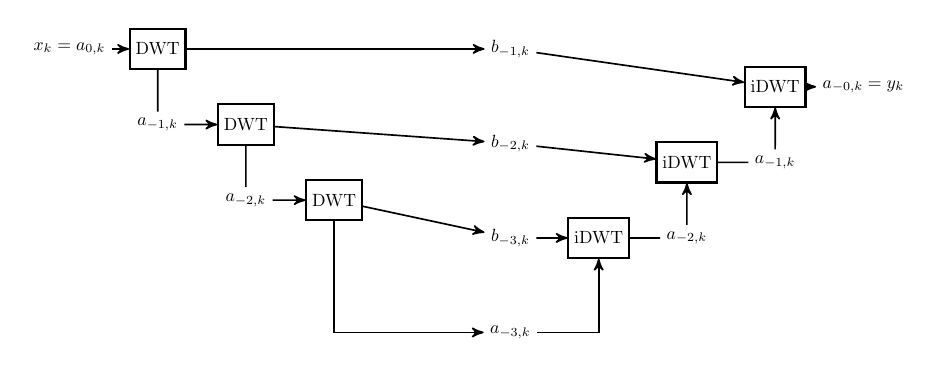
\begin{tikzpicture}[->, >=stealth', auto, semithick, node distance=1.5cm, scale = 0.8]

%\draw[step=1.0,black,thin,xshift=0.0cm,yshift=0.0cm] (-2,-8) grid (15,1);

%\useasboundingbox (0,-0.5) rectangle (12.5,1.5);

%\tikzset{every node/.style={scale=0.7}}

\tikzstyle{every state}=[fill=white,draw=black,thick,text=black,scale=0.8]
\tikzstyle{block}=[rectangle, inner sep=10pt, fill=white,draw=black,thick,text=black,scale=0.8]
\tikzstyle{square}=[rectangle, fill=white,draw=black,thick,text=black, minimum height = 0.8cm, minimum width = 0.8cm,scale=0.8]
\tikzstyle{round}=[circle, fill=white,draw=black,thick,text=black,scale=0.8]
\tikzstyle{dots}=[fill=white,thick,text=black,scale=0.8]

\node[dots] (a0) at (0,0) {$x_k = a_{0,k}$};

\node[square] (s1) [right of=a0, node distance=1.75cm] {DWT};
\node[dots] (b1) at (7 , 0) {$b_{-1,k}$};
\node[dots] (a1) [below of=s1] {$a_{-1,k}$};

\node[square] (s2) [right of=a1, node distance=1.75cm] {DWT};
\node[dots] (b2) at (7 , -1.5) {$b_{-2,k}$};
\node[dots] (a2) [below of=s2] {$a_{-2,k}$};

\node[square] (s3) [right of=a2, node distance=1.75cm] {DWT};
\node[dots] (b3) at (7 , -3) {$b_{-3,k}$};
\node[dots] (a3) at (7 , -4.5) {$a_{-3,k}$};

\node[square] (i3) [right of=b3, node distance=1.75cm] {iDWT};
\node[dots]   (ia3) [right of=i3, node distance=1.75cm] {$a_{-2,k}$};

\node[square] (i2) [above of=ia3] {iDWT};
\node[dots]   (ia2) [right of=i2, node distance=1.75cm] {$a_{-1,k}$};

\node[square] (i1) [above of=ia2] {iDWT};
\node[dots]   (ia1) [right of=i1, node distance=1.75cm] {$a_{-0,k} = y_k$};




\draw[->] (a0) -- (s1);
\draw[-] (s1) -- (a1);
\draw[->] (s1) -- (b1);


\draw[->] (a1) -- (s2);
\draw[-] (s2) -- (a2);
\draw[->] (s2) -- (b2);

\draw[->] (a2) -- (s3);
\draw[->] (s3) |- (a3);
\draw[->] (s3) -- (b3);

\draw[->] (a3) -| (i3);
\draw[->] (b3) -- (i3);
\draw[-] (i3) -- (ia3);

\draw[->] (ia3) -- (i2);
\draw[->] (b2) -- (i2);
\draw[-] (i2) -- (ia2);

\draw[->] (ia2) -- (i1);
\draw[->] (b1) -- (i1);
\draw[->] (i1) -- (ia1);



%
%\node[round] (d1) [right of=h1] {$\downarrow 2$};
%\node[round] (d2) [right of=h2] {$\downarrow 2$};
%
%\node[dots] (dots1) [right of=d1] {$a_{j,k} \- \text{(LP)}$};
%\node[dots] (dots2) [right of=d2] {$b_{j,k} \- \text{(HP)}$};
%
%\node[round] (u1) [right of=dots1] {$\uparrow 2$};
%\node[round] (u2) [right of=dots2] {$\uparrow 2$};
%
%\node[block] (hh1) [right of=u1] {$ h(z)$};
%\node[block] (hh2) [right of=u2] {$ g(z)$};
%
%\node[round] (combine) at (15,0) {$+$};
%
%\node[dots, right of=combine, node distance=1cm] (end) {$a_{j+1,k}$} ;

%\node[state]  (w1)          {$\omega_1$};
%
%\node[state]  (w0)    [left of=w1]                   {$\omega_0$};
%
%\node[state]  (w2)    [right of=w1]      {$\omega_2$};
%\node[dots]   (dotss) [right of=w2]      {...};
%\node[state]  (w5)    [right of=dotss]   {$\omega_5$};
%\node[state]  (w6)    [right of=w5]      {$\omega_6$};
%

c

%\draw[->] (split) |- node {}(h1);
%\draw[->] (split) |- node {}(h2);
%
%\draw[->] (h1) -- node {}(d1);
%\draw[->] (h2) -- node {}(d2);
%
%\draw[->] (d1) -- node {}(dots1);
%\draw[->] (d2) -- node {}(dots2);
%
%\draw[->] (dots1) -- node {}(u1);
%\draw[->] (dots2) -- node {}(u2);
%
%\draw[->] (u1) -- node {}(hh1);
%\draw[->] (u2) -- node {}(hh2);
%
%\draw[->] (hh1) -| node {}(combine);
%\draw[->] (hh2) -| node {}(combine);
%
%\draw[->] (combine) -- node {}(end);

%\path
%(start) edge[]       (split)
%     
%(split) edge[]     (w1);
%     
%(w1) edge[loop above]    node{$A_{1,1}$}     (w1)
%     edge[bend left]     node{$A_{1,2}$}     (w2)
%     
%(w2) edge[loop above]    node{$A_{2,2}$}     (w2)
%     edge[bend left]     node{$A_{2,3}$}     (dotss)
%
%(dotss) edge[bend left]    node{$A_{4,5}$}     (w5)
%     
%(w5) edge[loop above]    node{$A_{5,5}$}     (w5)
%     edge[bend left]     node{$A_{5,6}$}     (w6)
%     
%(w6) edge[loop above]    node{$A_{6,6}$}     (w6);


\end{tikzpicture}
	\caption{Tower of DWTs with 3 layers followed by a subsequent inverse transform tower.}
	\label{fpga:fig:dwtTower}
\end{figure}

\subsection{Lifting Scheme}

The lifting scheme is a technique to perform a DWT efficiently.
It was introduced in a paper by Ingrid Daubechies and Wim Sveldens \cite{fpga:Daubechies1998}. 
The lifting scheme is a widely used algorithm, which is more efficient in terms of the number of multiplications than normal wavelet transformations.
The number of arithmetic operations is reduced nearly by a factor of two compared to an ordinary, convolutional calculation.

The lifting scheme factorizes any discrete wavelet transform with finite filters into a series of elementary convolutions which are referred to as lifting steps.
This factorization splits a long filter into a tree of small filters, which is numerically superior in terms of rounding errors.
This decomposition is equivalent to a factorization of the polyphase matrix of the wavelet filter into elementary matrices, as elaborated in the following sections.

%In this paper, we want to focus only on orthogonal wavelets, where $\bm h = \bm{\bar h}$ and $\bm g = \bm{\bar g}$.
In order to be consistent with the paper, we use the terminology of Daubechies et al. who refer to the coefficients
\begin{align}
\bm a & \leftrightarrow \bm s \quad \text{(smooth)} \quad \text{and} \\
\bm b & \leftrightarrow \bm d \quad \text{(detail)} .
\end{align}

\subsubsection{Polyphase Decomposition \label{fpga:polyphase}}

The lifting scheme takes advantage of the polyphase decomposition, which is broadly applied when downsampling or upsampling is used. 
The scaling relation leads to a downsampling factor of two.
This corresponds to splitting the signal into a channel for even samples $e$ and a channel for odd samples $o$.
The polyphase decomposition splits an algebraic expression into one part for each channel, which are also referred to as the polyphase components.
%The polyphase components are the filter components of the sub channels.
In order to continue in a polyphase implementation, all data, including the filter coefficients, must be split as well.
This process is demonstrated with the $\bm h$ filter coefficients.
Its polyphase decomposition is
\begin{equation}
	h(z) = \sum_{n=-\infty}^{\infty} h_{2n} z^{-2n} + z^{-1} \sum_{n=-\infty}^{\infty} h_{2n+1} z^{-2n},
\end{equation}
or in the z-domain:
\begin{equation}
	h(z)=h_{e}(z^2) + z^{-1} h_o(z^2),
\end{equation}
where $h_o(z^2)$ is the two times upsampled version of $h_o(z)$.
This yields the even and odd components:
\begin{align}
	h_e(z) &= \sum_{n=-\infty}^{\infty} h_{2n} z^{-n}
	\\
	h_o(z) &= \sum_{n=-\infty}^{\infty} h_{2n+1} z^{-n}.
\end{align}
These coefficients are then placed together with the $g(z)$ components in the polyphase matrix
\begin{equation}
	\bm P(z) = 
	\begin{bmatrix}
	h_e(z) & g_e(z) \\
	h_o(z) & g_o(z)
	\end{bmatrix}.
\end{equation}
Using the polyphase decomposition the DWT algorithm is
\begin{align}
\begin{bmatrix}
	s(z) \\
	d(z)
\end{bmatrix}
&=
\bm{\bar P}(z^{-1})^t
\begin{bmatrix}
	x(z^2) \\     
	x(z^2) z
\end{bmatrix}
\\
\begin{bmatrix}
	y(z^2) \\
	y(z^2) z
\end{bmatrix}
&=
\bm P(z)
\begin{bmatrix}
	s(z) \\
	d(z)
\end{bmatrix}
,
\end{align}
where $x$ is the input of the forward DWT and $y$ is the reconstructed output of the inverse DWT.
The DWT using polyphase implementation is depicted graphically in figure \ref{fpga:fig:liftingSteps}.
\begin{figure}
	\centering
	\usetikzlibrary{automata,arrows,positioning,calc}



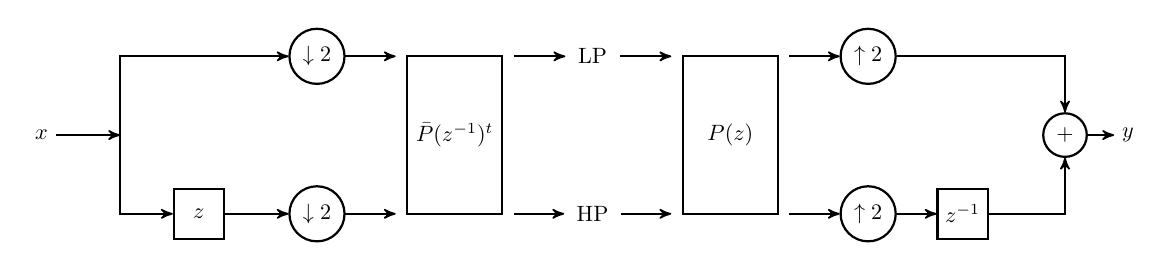
\begin{tikzpicture}[->, >=stealth', auto, semithick, node distance=1.5cm, scale = 1]


%\useasboundingbox (0,-0.5) rectangle (12.5,1.5);

%\tikzset{every node/.style={scale=0.7}}

\tikzstyle{block}=[rectangle, inner sep=4pt, fill=white,draw=black,thick,text=black, minimum height = 2.5cm, minimum width = 1.5cm, scale = 1]
\tikzstyle{square}=[rectangle, fill=white,draw=black,thick,text=black, minimum height = 0.8cm, minimum width = 0.8cm,  scale = 1]
\tikzstyle{round}=[circle, fill=white,draw=black,thick,text=black,  scale = 1]
\tikzstyle{dots}=[circle, fill=white,thick,text=black,scale=1, minimum size=0.8cm,  scale = 1]

%\draw[step=1.0,black,thin,xshift=0.0cm,yshift=0.0cm] (-2,-3) grid (10,3);

%\tikzset{every node/.style={scale=0.7}}

\node      (start) at(0,0) {$x$} ;

\coordinate (split)  at(1,0);

\node[] (z1)  {};
\node[square] (z2) at (2,-1) {$z$};

\node[round] (d1) at (3.5,1) {$\downarrow 2$};
\node[round] (d2) at (3.5,-1) {$\downarrow 2$};

\coordinate (h1tl) at (4.5, 1);
\coordinate (h1bl) at (4.5,-1);
\coordinate (h1tr) at (6, 1);
\coordinate (h1br) at (6,-1);
\node[block] (h1) at (5.25,0) {$\bm{\bar P}(z^{-1})^t$};



\node[dots] (dots1) at (7, 1) {\text{LP}};
\node[dots] (dots2) at (7, -1) {\text{HP}};

\coordinate (h2tl) at (8, 1);
\coordinate (h2bl) at (8,-1);
\coordinate (h2tr) at (9.5, 1);
\coordinate (h2br) at (9.5,-1);
\node[block] (h2) at (8.75,0) {$\bm P(z)$};


\node[round] (u1) at (10.5,1) {$\uparrow 2$};
\node[round] (u2) at (10.5,-1) {$\uparrow 2$};

\node[] (zz1) [right of=u1] {};
\node[square] (zz2) [right of=u2] {$z^{-1}$};

\node[round] (combine)  at (13,0){$+$};

\node[right of=combine, node distance=1cm] (end) {$y$};


\draw[->] (start) -- node {}(split);

\draw[->] (split) |- node {}(d1);
\draw[->] (split) |- node {}(z2);
\draw[->] (z2) -- node {}(d2);

\draw[->] (d1) -- node {}(h1tl);
\draw[->] (d2) -- node {}(h1bl);

\draw[->] (h1tr) -- node {}(dots1);
\draw[->] (h1br) -- node {}(dots2);

\draw[->] (dots1) -- node {}(h2tl);
\draw[->] (dots2) -- node {}(h2bl);

\draw[->] (h2tr) -- node {}(u1);
\draw[->] (h2br) -- node {}(u2);



\draw[->] (u1) -| node {}(combine);
\draw[->] (u2) -- node {}(zz2);
\draw[->] (zz2) -| node {}(combine);

\draw[->] (combine) -- node {}(end);


\end{tikzpicture}
	\caption{DWT graph using the polyphase matrix $\bm P$}
	\label{fpga:fig:liftingSteps}
\end{figure}

\section{Lifting}
\rhead{Lifting}

The core idea of the polyphase decomposition is the possibility of factorizing the $\bm P$ matrix.
Daubechies et al. prove that this is possible for an arbitrary complementary matrix $\bm P$ if composed only of Laurent polynomials.
The factorization algorithm is not explained in this work, since the required theory exceeds what is covered in part 1.
However, it results in the form
\begin{align}
	\bm{\bar P}(z) &=
	\Biggl(
	\prod_{i=1}^{m}
	\begin{bmatrix}
		1 & 0 \\
		-s_i(z^{-1}) & 1
	\end{bmatrix}
	\begin{bmatrix}
		1 & -t_i(z^{-1}) \\
		0 & 1
	\end{bmatrix}
	\Biggr)
	\begin{bmatrix}
		\frac{1}{K} & 0 \\
		0 & K
	\end{bmatrix}
	\\
	\bm P(z) &=
	\Biggl(
	\prod_{i=1}^{m}
	\begin{bmatrix}
		1 & s_i(z) \\
		0 & 1
	\end{bmatrix}
	\begin{bmatrix}
		1 & 0 \\
		t_i(z) & 1
	\end{bmatrix}
	\Biggr)
	\begin{bmatrix}
		K & 0 \\
		0 & \frac{1}{K}
	\end{bmatrix}
	.
\end{align}
The factorized matrices consist of $1$ in the diagonal and one single factor in the upper right or lower left corner.
A matrix of this structure only uses one multiplication and one addition to implement, which results in sort of a ladder structure.
Figure \ref{fpga:fig:liftingStepFactorization} shows a graphical version of the factorized DWT.
The implementation uses only $2(i+1)$ multiplications and $2i$ additions.
Hence, it is two times more efficient than the convolutional DWT.
\begin{figure}
	\centering
	%\includeagraphics[width=\hsize]{papers/fpga/tikz/liftingStepFactorization.tikz}
	\usetikzlibrary{automata,arrows,positioning,calc}
\usetikzlibrary{shapes}

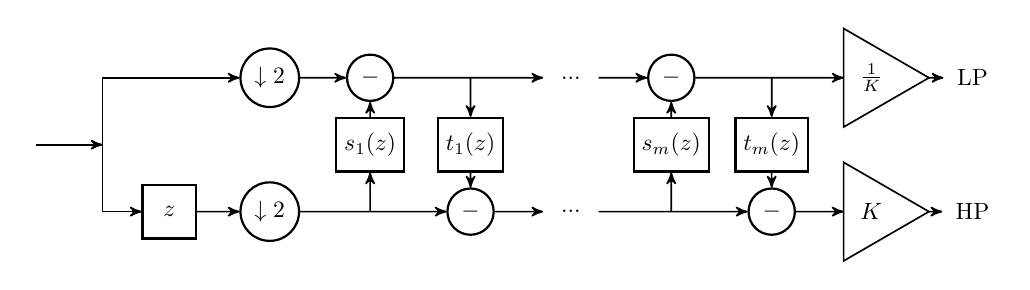
\begin{tikzpicture}[->, >=stealth', auto, semithick, node distance=1.5cm, scale = 0.85]

%\useasboundingbox (0,-0.5) rectangle (12.5,1.5);

\tikzstyle{block}=[rectangle, inner sep=4pt, fill=white,draw=black,thick,text=black, minimum height = 2.5cm, minimum width = 1.5cm, scale = 1]
\tikzstyle{square}=[rectangle, fill=white,draw=black,thick,text=black, minimum height = 0.8cm, minimum width = 0.8cm,  scale = 1]
\tikzstyle{round}=[circle, fill=white,draw=black,thick,text=black, scale = 1]
\tikzstyle{dots}=[circle, fill=white,thick,text=black, minimum size=0.8cm,  scale = 1]
\tikzstyle{amp}= [regular polygon, regular polygon sides=3,	draw, fill=white, text width=1em, inner sep=0.5mm, outer sep=0mm,	shape border rotate=-90, minimum size = 1.7cm, scale = 1]

\tikzset{every node/.style={scale=0.85}}
\tikzset{every coordinate/.style={scale=0.85}}

%\draw[step=1.0,black,thin,xshift=0.0cm,yshift=0.0cm] (-2,-3) grid (10,3);

\coordinate (start) at(0,0) ;

\coordinate (split)  at(1,0);

\node[] (z1)  {};
\node[square] (z2) at (2,-1) {$z$};

\node[round] (d1) at (3.5,1) {$\downarrow 2$};
\node[round] (d2) at (3.5,-1) {$\downarrow 2$};

\node[round] (min1) [right of=d1] {$-$};
\node[square] (s1) [below of=min1, node distance=1cm] {$s_1(z)$};
\coordinate[right of=d2] (c1) ;

\node[round] (min2) [right of=c1] {$-$};
\node[square] (s2) [above of=min2, node distance=1cm] {$t_1(z)$};
\coordinate[right of=min1] (c2) [right of=min1];

\node[dots] (dots1) [right of=c2] {...};
\node[dots] (dots2) [right of=min2] {...};

\node[round] (min3) [right of=dots1] {$-$};
\node[square] (s3) [below of=min3, node distance=1cm] {$s_m(z)$};
\coordinate[right of=dots2] (c3) ;

\node[round] (min4) [right of=c3] {$-$};
\node[square] (s4) [above of=min4, node distance=1cm] {$t_m(z)$};
\coordinate[right of=min3] (c4) [right of=min1];

\node[amp] (amp1) [right of=c4] {$\frac{1}{K}$};
\node[amp] (amp2)  [right of=min4] {$K$};

\node[dots] (lp) [right of=amp1] {\text{LP}};
\node[dots] (hp) [right of=amp2] {\text{HP}};


\draw[->] (start) -- (split);

\draw[->] (split) |- (d1);
\draw[->] (split) |- (z2);
\draw[->] (z2) -- (d2);


\draw[->] (d1) -- (min1);
\draw[->] (d2) -- (min2);

\draw[->] (c1) -- (s1);
\draw[->] (s1) -- (min1);
\draw[->] (c2) -- (s2);
\draw[->] (s2) -- (min2);

\draw[->] (min1) -- (dots1);
\draw[->] (min2) -- (dots2);


\draw[->] (dots1) -- (min3);
\draw[->] (dots2) -- (min4);

\draw[->] (c3) -- (s3);
\draw[->] (s3) -- (min3);
\draw[->] (c4) -- (s4);
\draw[->] (s4) -- (min4);

\draw[->] (min3) -- (amp1);
\draw[->] (min4) -- (amp2);

\draw[->] (amp1) -- (lp);
\draw[->] (amp2) -- (hp);

\end{tikzpicture}
	\usetikzlibrary{automata,arrows,positioning,calc}
\usetikzlibrary{shapes}

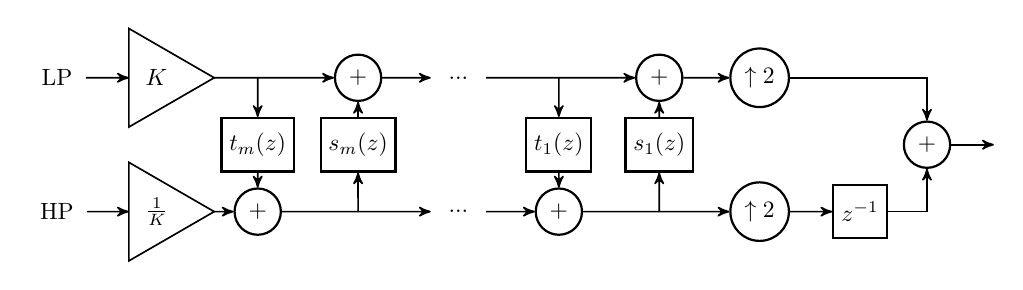
\begin{tikzpicture}[->, >=stealth', auto, semithick, node distance=1.5cm, scale = 0.85]

%\useasboundingbox (0,-0.5) rectangle (12.5,1.5);

\tikzstyle{block}=[rectangle, inner sep=4pt, fill=white,draw=black,thick,text=black, minimum height = 2.5cm, minimum width = 1.5cm, scale = 1]
\tikzstyle{square}=[rectangle, fill=white,draw=black,thick,text=black, minimum height = 0.8cm, minimum width = 0.8cm,  scale = 1]
\tikzstyle{round}=[circle, fill=white,draw=black,thick,text=black,  scale = 1]
\tikzstyle{dots}=[circle, fill=white,thick,text=black,scale=1, minimum size=0.8cm,  scale = 1]
\tikzstyle{amp}= [regular polygon, regular polygon sides=3,	draw, fill=white, text width=1em, inner sep=0.5mm, outer sep=0mm,	shape border rotate=-90, minimum size = 1.7cm, scale = 1]

\tikzset{every node/.style={scale=0.85}}
\tikzset{every coordinate/.style={scale=0.85}}

%\draw[step=1.0,black,thin,xshift=0.0cm,yshift=0.0cm] (-2,-3) grid (10,3);

\node[dots] (lp) at (0,1) {\text{LP}};
\node[dots] (hp) at (0,-1) {\text{HP}};

\node[amp] (amp1) [right of=lp] {$K$};
\node[amp] (amp2) [right of=hp] {$\frac{1}{K}$};


\coordinate[right of=amp1] (c1) ;
\node[round] (sum1) [right of=amp2] {$+$};
\node[square] (s1) [above of=sum1, node distance=1cm] {$t_m(z)$};

\coordinate[right of=sum1] (c2) ;
\node[round] (sum2) [right of=c1] {$+$};
\node[square] (s2) [below of=sum2, node distance=1cm] {$s_m(z)$};


\node[dots] (dots1) [right of=sum2] {...};
\node[dots] (dots2) [right of=c2] {...};


\coordinate[right of=dots1] (c3) ;
\node[round] (sum3) [right of=dots2] {$+$};
\node[square] (s3) [above of=sum3, node distance=1cm] {$t_1(z)$};

\coordinate[right of=sum3] (c4) ;
\node[round] (sum4) [right of=c3] {$+$};
\node[square] (s4) [below of=sum4, node distance=1cm] {$s_1(z)$};


\node[round] (u1) [right of=sum4] {$\uparrow 2$};
\node[round] (u2) [right of=c4] {$\uparrow 2$};

\node[square] (zz2) [right of=u2] {$z^{-1}$};

\node[round] (combine)  at (13,0){$+$};

\coordinate[right of=combine, node distance=1cm] (end);

\draw[->] (lp) -- (amp1);
\draw[->] (hp) -- (amp2);


\draw[->] (amp1) -- (sum2);
\draw[->] (amp2) -- (sum1);

\draw[->] (c1) -- (s1);
\draw[->] (s1) -- (sum1);
\draw[->] (c2) -- (s2);
\draw[->] (s2) -- (sum2);

\draw[->] (sum2) -- (dots1);
\draw[->] (sum1) -- (dots2);


\draw[->] (dots1) -- (sum4);
\draw[->] (dots2) -- (sum3);

\draw[->] (c3) -- (s3);
\draw[->] (s3) -- (sum3);
\draw[->] (c4) -- (s4);
\draw[->] (s4) -- (sum4);

\draw[->] (sum4) -- (u1);
\draw[->] (sum3) -- (u2);


\draw[->] (u1) -| (combine);
\draw[->] (u2) -- (zz2);
\draw[->] (zz2) -| (combine);

\draw[->] (combine) -- (end);

\end{tikzpicture}
	\caption{DWT signal flow graph with factorized filter functions (lifting steps)}
	\label{fpga:fig:liftingStepFactorization}
\end{figure}
$\bm s(z)$ and $\bm t(z)$ result from the factorizing algorithm.
They replace $\bm h(z)$ and $\bm g(z)$ completely.

\subsection{Haar wavelet}
\label{fpga:sec:haar}

For the sake of simplicity, we initially chose the unnormalized Haar wavelet for the VHDL implementation, which consists of the following coefficients:
\begin{align}
	h(z) = 1 + z^{-1} \quad & \Rightarrow \quad \bar h(z) = \frac{1}{2} + \frac{1}{2} z^{-1}
	\\
	g(z) = - \frac{1}{2} + \frac{1}{2} z^{-1} \quad & \Rightarrow \quad \bar g(z) = -1 + z^{-1}
\end{align}
If these coefficients are split into even and odd components and filled into the polyphase matrix we get for the forward transform
\begin{equation*}
	\bm {\bar P}(z^{-1})^t =
	\begin{bmatrix}
		\frac{1}{2} & \frac{1}{2} \\
		-1 & 1
	\end{bmatrix}
	= 
	\begin{bmatrix}
		1 & \frac{1}{2} \\
		0 & 1
	\end{bmatrix}
	\cdot
	\begin{bmatrix}
		1 & 0 \\
		-1 & 1
	\end{bmatrix}
	.
\end{equation*}
The term on the right side is a possible factorization which results in lifting steps.
The factorization produces diagonal lifting step matrices, which are easy to compute.
This corresponds to the following pseudo code for a forward transform \cite{fpga:Daubechies1998}:
\begin{align}\label{fpga:equation:haar}
	s_l^{(0)} &= x_{2l} \\
	d_l^{(0)} &= x_{2l+1} \\ 
	d_l &= d_l^{(0)} - s_l^{(0)} \\
	s_l &= s_l^{(0)} + \frac{1}{2}d_l
	,
\end{align}
where $x_{n}$ is the incoming sample stream.
The analysis side is in the following form:
\begin{equation*}
	\bm P(z) =
	\begin{bmatrix}
		1 & -\frac{1}{2} \\
		1 & \frac{1}{2}
	\end{bmatrix}
	= 
	\begin{bmatrix}
		1 & 0 \\
		1 & 1
	\end{bmatrix}
	\cdot
	\begin{bmatrix}
		1 & -\frac{1}{2} \\
		0 & 1
	\end{bmatrix}
	.
\end{equation*}
In this case the inverse transformation is 
\begin{align}\label{fpga:equation:inv_haar}
	s_l^{(0)} &= s_l - \frac{1}{2}d_l \\
	d_l^{(0)} &= d_l + s_l \\ 
	x_{2l+1}& =d_l^{(0)} \\
	x_{2l} &= s_l^{(0)}
\end{align}
and the original stream can be fully recovered.
Figure \ref{fpga:fig:liftingStepHaar} shows both transforms graphically.
\begin{figure}
	\centering
	\usetikzlibrary{automata,arrows,positioning,calc}
\usetikzlibrary{shapes}


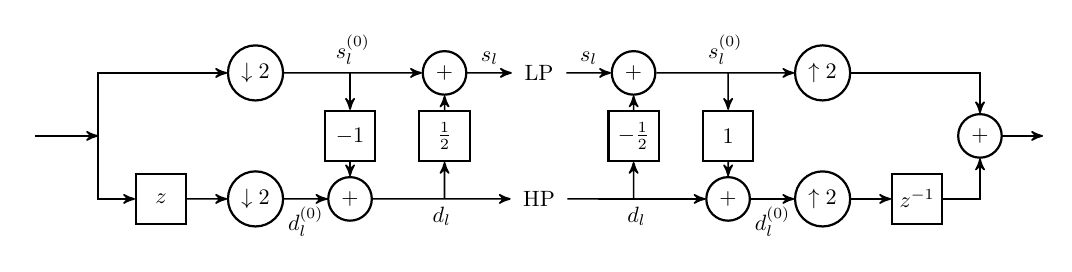
\begin{tikzpicture}[->, >=stealth', auto, semithick, node distance=1.5cm, scale = 0.8]


%\useasboundingbox (0,-0.5) rectangle (12.5,1.5);



\tikzstyle{block}=[rectangle, inner sep=4pt, fill=white,draw=black,thick,text=black, minimum height = 2.5cm, minimum width = 1.5cm, scale = 1]
\tikzstyle{square}=[rectangle, fill=white,draw=black,thick,text=black, minimum height = 0.8cm, minimum width = 0.8cm,  scale = 1]
\tikzstyle{round}=[circle, fill=white,draw=black,thick,text=black,  scale = 1]

\tikzstyle{dots}=[circle, fill=white,thick,text=black,scale=1, minimum size=0.8cm,  scale = 1]

\tikzstyle{amp}= [regular polygon, regular polygon sides=3,	draw, fill=white, text width=1em, inner sep=0.5mm, outer sep=0mm, shape border rotate=-90, minimum size = 1.7cm, scale = 1]

\tikzset{every node/.style={scale=0.8}}
\tikzset{every coordinate/.style={scale=0.8}}

%\draw[step=1.0,black,thin,xshift=0.0cm,yshift=0.0cm] (-2,-3) grid (10,3);

%\tikzset{every node/.style={scale=0.7}}

\coordinate      (start) at(0,0) ;

\coordinate (split)  at(1,0);

\node[] (z1)  {};
\node[square] (z2) at (2,-1) {$z$};

\node[round] (d1) at (3.5,1) {$\downarrow 2$};
\node[round] (d2) at (3.5,-1) {$\downarrow 2$};



\node[round] (sum1) [right of=d2] {$+$};
\node[square] (s1) [above of=sum1, node distance=1cm] {$-1$};
\coordinate[right of=d1] (c1);

\node[round] (sum2) [right of=c1] {$+$};
\node[square] (s2) [below of=sum2, node distance=1cm] {$\frac{1}{2}$};
\coordinate[right of=sum1] (c2) ;

\node[dots] (hp) [right of=sum2] {\text{LP}};
\node[dots] (lp) [right of=c2]   {\text{HP}};



\coordinate[right of=lp] (c3);
\node[round] (sum3) [right of=hp] {$+$};
\node[square] (s3) [below of=sum3, node distance=1cm] {$-\frac{1}{2}$};

\coordinate[right of=sum3] (c4) ;
\node[round] (sum4) [right of=c3] {$+$};
\node[square] (s4) [above of=sum4, node distance=1cm] {$1$};


\node[round] (u1) [right of=c4] {$\uparrow 2$};
\node[round] (u2) [right of=sum4] {$\uparrow 2$};

\node[square] (zz2) [right of=u2] {$z^{-1}$};

\node[round] (combine)  at (15,0){$+$};

\coordinate[right of=combine, node distance=1cm] (end);


\draw[->] (start) -- (split);

\draw[->] (split) |- (d1);
\draw[->] (split) |- (z2);
\draw[->] (z2) -- (d2);


\draw[->] (d1) -- node[above]{$s_l^{(0)}$} (sum2);
\draw[->] (d2) -- node[below]{$d_l^{(0)}$} (sum1);

\draw[->] (c1) -- (s1);
\draw[->] (s1) -- (sum1);
\draw[->] (c2) -- (s2);
\draw[->] (s2) -- (sum2);

\draw[->] (sum2) -- node[above]{$s_l$} (hp);
\draw[->] (sum1) -- node[below]{$d_l$} (lp);

\draw[->] (hp) -- node[above]{$s_l$} (sum3);
\draw[->] (lp) -- node[below]{$d_l$} (sum4);



\draw[->] (c3) -- (s3);
\draw[->] (s3) -- (sum3);
\draw[->] (c4) -- (s4);
\draw[->] (s4) -- (sum4);

\draw[->] (sum3) -- node[above]{$s_l^{(0)}$}(u1);
\draw[->] (sum4) -- node[below]{$d_l^{(0)}$}(u2);


\draw[->] (u1) -| (combine);
\draw[->] (u2) -- (zz2);
\draw[->] (zz2) -| (combine);

\draw[->] (combine) -- (end);


\end{tikzpicture}
	\caption{Lifting scheme implementation of the Haar wavelet.}
	\label{fpga:fig:liftingStepHaar}
\end{figure}

\section{VHDL Implementation}
\rhead{VHDL Implementation}

The VHDL implementation adds some complexity to the mathematical representation of the algorithm.
A physical implementation allows only causal filters.
In other words, a filter may only use information of the past and not the future.
These are recognizable by containing solely negative powers of $z$.
All non-causal filters must be delayed, in order to get causal.
Notably, the polyphase decomposition of the forward wavelet transform is non-causal and must be delayed by one sample.

\subsection{Design Considerations}

When implementing an algorithm in hardware, a lot of design considerations must be made in advance.
The hardware architecture is very dependent of the application.
A hardware block can be optimized for various goals, such as high accuracy, low latency, high data rate, low area and low power consumption.
Since this work is not based on a defined objective, we must come up with our own design specifications.

In most cases which do not require low latency and high data rates, a digital signal processor would be a better choice than a custom VHDL-implemented hardware.
A sequential processor unit is computationally very efficient and requires almost no chip area compared to most VHDL solutions.
However, it features a significantly higher latency, which is a major drawback.
Hence, the VHDL implementation should feature low latency and high data rate as its main objectives in order to provide a solution which is useful as a hardware implementation.
The application should make use of one of the biggest advantages of custom hardware, which is parallelism.
Performing calculations in parallel leads to higher throughput and allows data rates which are as fast as the clock speed of the logic.
The strengths of the chosen implementation are thus high speed and low latency processing suitable for real-time applications.

Implementing the Haar wavelet has been the main priority.
A optional goal has been the implementation of a higher order wavelet, such as the orthogonal Daubechies-4 wavelet.
The implementation should be as generic as possible, in order to allow customization.

\subsection{Idea}

A forward and inverse multiresolution analysis DWT should be implemented, where each function is contained in a VHDL entity.
Figure \ref{fpga:fig:idea} shows the outline of the two blocks.
\begin{figure}
	\centering
	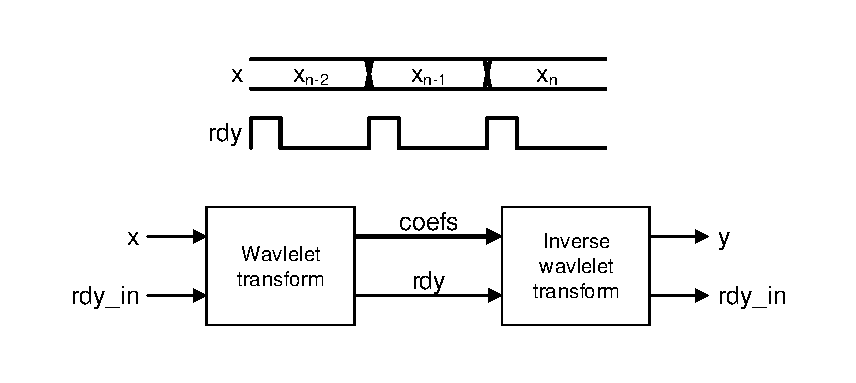
\includegraphics[width=0.8\textwidth]{papers/fpga/images/idea.pdf}
	\caption{Outline of the modules \label{fpga:fig:idea}}
\end{figure}
The number of multiresolution layers $N$ can be specified as a generic parameter.
The forward algorithm has a 16-bit signed number input \texttt{x} ($a_{j,k} \forall k=0$) and outputs the wavelet coefficients as a stream.
The input is accompanied by a ready signal, which determines the sample rate of the input.
This signal must be driven \texttt{1} when a sample is to be processed and \texttt{0} otherwise.
If it is always driven \texttt{1}, the input value is sampled continuously at each clock cycle.
The output coefficients are in form of a vector \texttt{d\_s}, which holds $N$ detail coefficients ($b_{j,*} \forall j \in [-1 .. -N]$) and \texttt{s}, which holds the remaining smooth coefficient ($a_{j,*} \forall j = -N$).
Each coefficient is 16 bits wide.
The coefficients are accompanied by a vector of output ready signals with length $N$, where each element corresponds to a level of the multiresolution analysis.
These signals are required to pass the phase information of the coefficients to a connecting block.
If the coefficient is updated, the ready signal is driven \texttt{1}, similar to the input ready signal.

%The inverse wavelet transform \texttt{inv\_haar} has an analogous outline.
The inverse DWT interface is defined as the forward DWT, with its inputs and outputs swapped.
It has the coefficients and ready signals as input and outputs the reconstructed signal \texttt{y}, again accompanied by its ready signal.

\subsection{Architecture}

The following sections describe the internal blocks in detail.
Figure \ref{fpga:fig:mainDelay} depicts an overview of the forward and inverse blocks.
\begin{figure} %TODO add clarification forward dwt = branching...
	\centering
	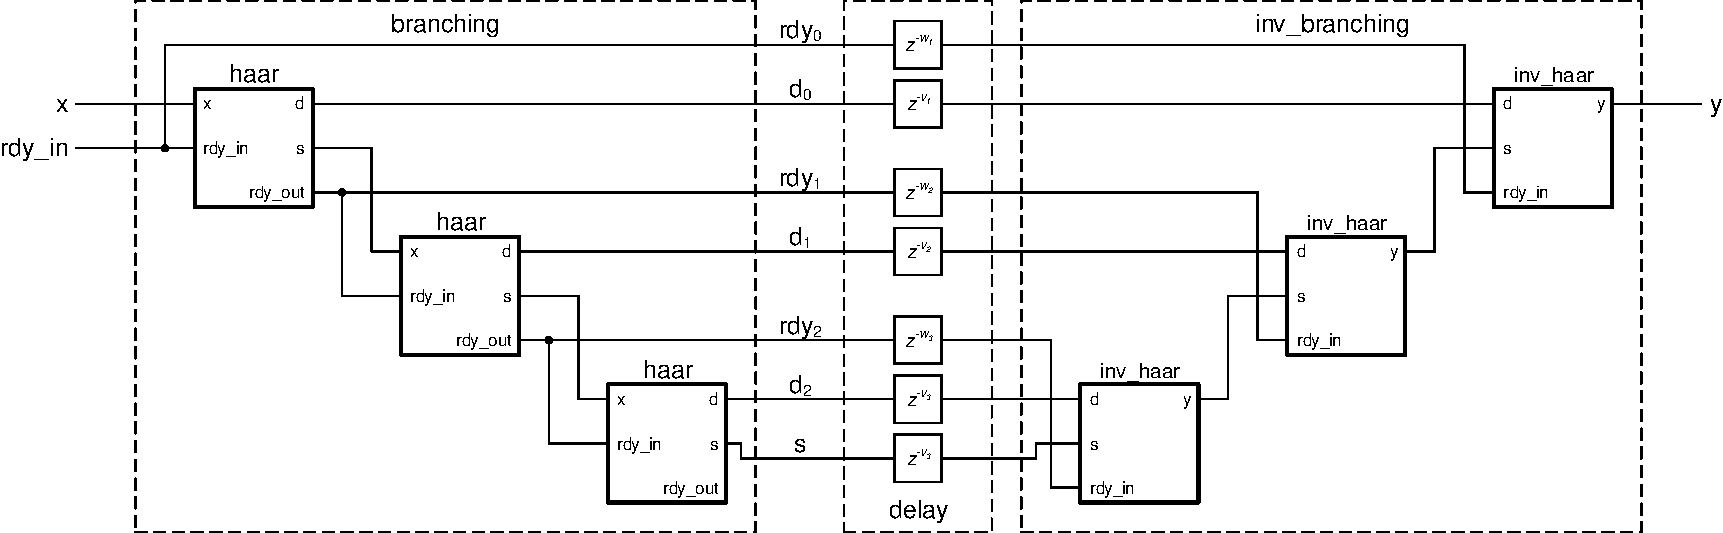
\includegraphics[width=\textwidth]{papers/fpga/images/main_delay.pdf}
	\caption{Complete architecture \label{fpga:fig:mainDelay}}
\end{figure}
In this formation the input \texttt{x} is converted into wavelet coefficients and subsequently reconstructed to the output \texttt{y}.
Thanks to lossless reconstruction, \texttt{y} is equal to \texttt{x} if delayed with the latency of the blocks, within numerical accuracy.

\subsubsection{Wavelet transform}

The transformation block \texttt{haar} implements the algorithm needed for the Haar DWT.
So far, only the Haar wavelet has been implemented.
Yet, the outline stays the same for every other discrete wavelet and allows a later implementation of more wavelets.
Figure \ref{fpga:fig:haar} shows the interface of the \texttt{haar} and \texttt{inv\_haar} block.
\begin{figure}
	\centering
	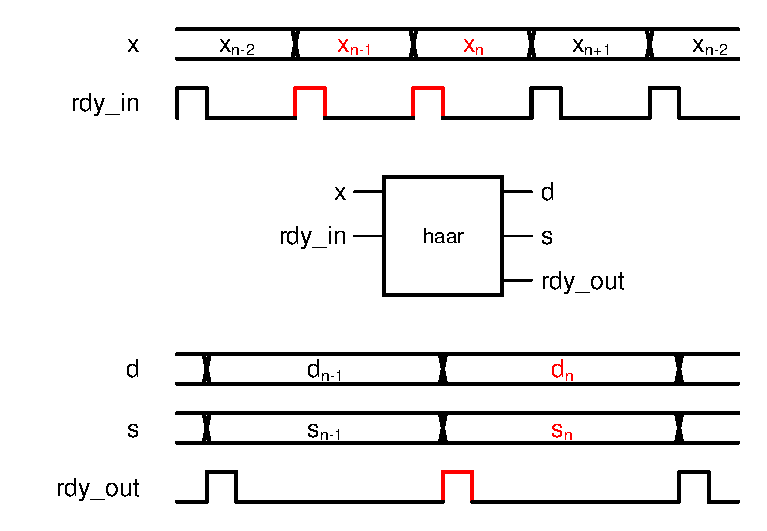
\includegraphics[width=0.49\textwidth]{papers/fpga/images/haar.pdf} %TODO fix rdy signal
	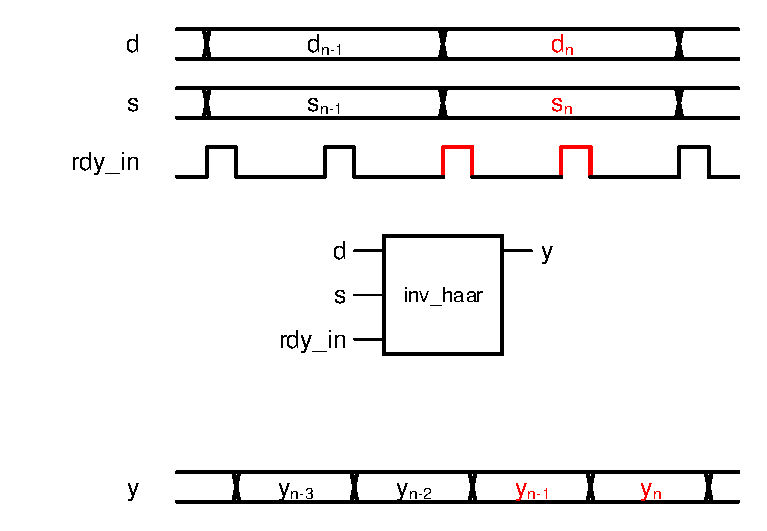
\includegraphics[width=0.49\textwidth]{papers/fpga/images/inv_haar.pdf}
	\caption{Interface description of the forward and inverse Haar wavelet blocks. \label{fpga:fig:haar}}
\end{figure}
The arithmetics inside the blocks are implemented as derived in section \ref{fpga:sec:haar}.
In the case of the Haar wavelet, the arithmetic is a fairly simple sequence of calculations as described in equation \ref{fpga:equation:haar}.
Multiplications and divisions by a factor of 2 are efficiently implemented with a bit shift in either direction.
The output of the \texttt{haar} block features the half sample rate due to the down sampling operator.
The forward transform, which is in mathematical notation non-causal, has been delayed in order to become causal.
In order to contain the propagation delay, registers (flip-flops) have been inserted for all output signals of the \texttt{haar} and \texttt{inv\_haar} blocks.
This leads to an additional delay of one clock cycle.
If longer wavelets than the Haar wavelet were to be implemented, more registers stages are required in order to avoid timing problems. %TODO grammar?

\subsubsection{Multiresolution analysis}

The multiresolution analysis is achieved by chaining the wavelet transform blocks.
The blocks which holds the multiresolution analysis are called \texttt{branching} and \texttt{inv\_branching}.
Each hold $N$ \texttt{haar} or \texttt{inv\_haar} blocks respectively, which are connected accordingly.

\subsubsection{Delay \label{fpga:sec:delay}}

The \texttt{branching} and \texttt{inv\_branching} block are sufficient for an independent forward or inverse transform.
However, the output of the forward transform and the input of the inverse transform are not compatible if applied to the same stream.
A direct connection of the two blocks shifts the coefficients out of phase, which results in a faulty interpretation of the signals.
This behavior is mostly due to the exponentially growing delay caused by the causal implementation of the polyphase decomposition.
In order to make the blocks connectable, a delay block must be inserted in between of the two blocks.
Figure \ref{fpga:fig:delay} compares the ready signals of the forward DWT output coefficients and the inverse DWT input coefficients.
Clearly, they are not in sync.
\begin{figure}
	\centering
	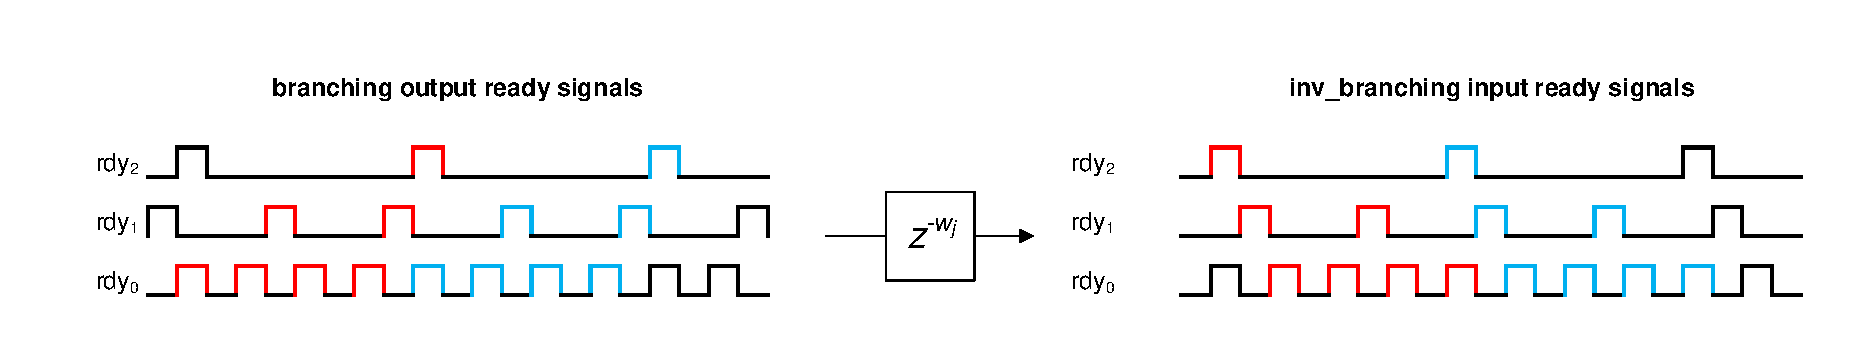
\includegraphics[width=\hsize]{papers/fpga/images/delay.pdf}
	\caption{
		Shift between the ready signals of the forward and inverse branching blocks.
	}
	\label{fpga:fig:delay}
\end{figure}
Each coefficient needs to be delayed individually, in order to match the interface of the inverse block.
The high frequency coefficients need to be delayed longer, whereas the lower coefficients only need a short delay.
The coefficient with the lowest frequency can be used without a delay.
The coefficients are delayed using a FIFO (first in - first out) buffer, while the ready signals are delayed in a with cascaded flip-flops.
A higher order wavelet would result in more latency and requires different delays. 

\subsection{Testing}

The test structure contains the forward transform, followed by the inverse transform, which should recover the original signal from the processed coefficients.
The test setup is shown in figure \ref{fpga:fig:testing}.
\begin{figure}
	\centering
	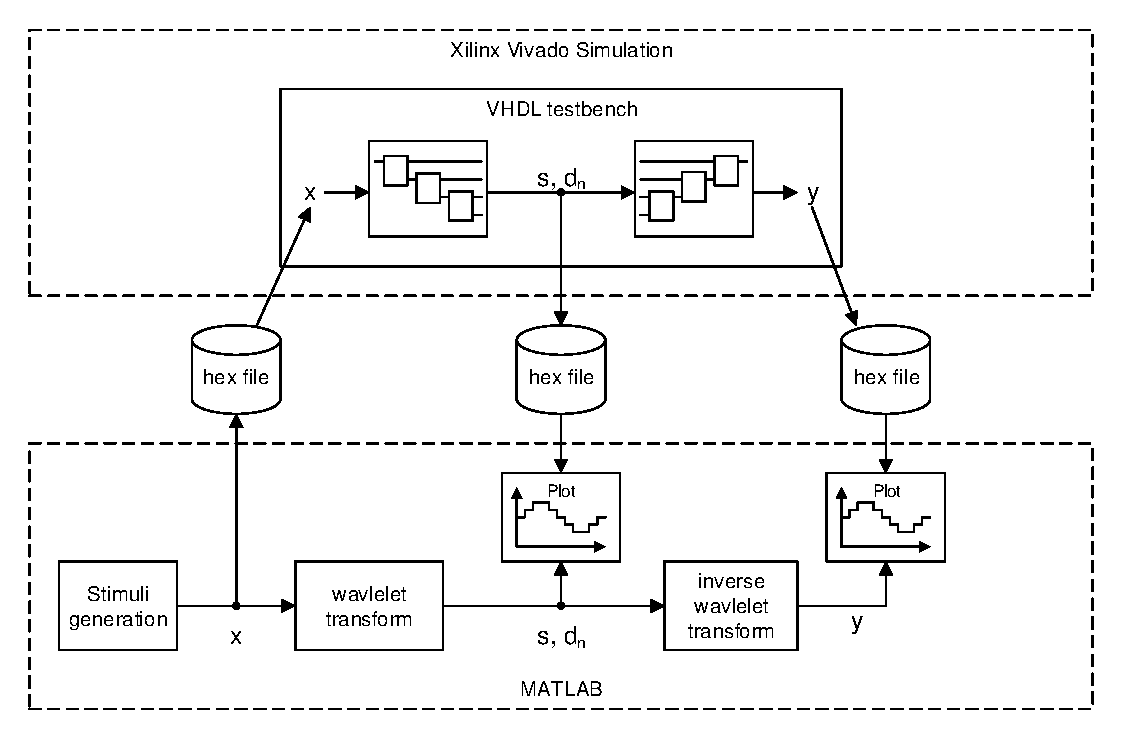
\includegraphics[width=\textwidth]{papers/fpga/images/vhdl_sim.pdf}
	\caption{Testing Workflow \label{fpga:fig:testing}}
\end{figure}
If no mistakes are present, the output should resemble the input, delayed by the latency of the whole pipeline.
The Vivado toolchain by Xilinx has been used to simulate the VHDL modules.
The wavelet transforms have also been implemented using integer numbers in MATLAB in order to provide a direct comparison.
An important point is to round towards negative infinity when performing divisions.
This leads to divisions which are numerically identical to integer divisions in hardware.
In MATLAB, this is accomplished with the function \texttt{idivide(x, 'floor')} instead of using the normal division operator (\texttt{/}).
A set of helper modules have been implemented in VHDL 2008, which are able to read and write test vectors and results from or to a file.
These modules provide an easy way to inject test data from the MATLAB enviroment.
After the VHDL simulation finishes, the results are again fed into MATLAB for validation.

\section{Results}
\rhead{Results}

After some testing and debugging the plots are promising.
The results of the extracted data from the Vivado toolchain and the numerical equivalent MATLAB simulation match up.
To compare every step of the processed data, the signals are extracted after transformation, after delaying and finally after the reconstruction.
The different signal stages are then plotted in MATLAB and compared.

In figure \ref{fpga:fig:coeff} shows the plotted coefficients after the forward transformation, but before the delay block
\begin{figure}
	\centering
	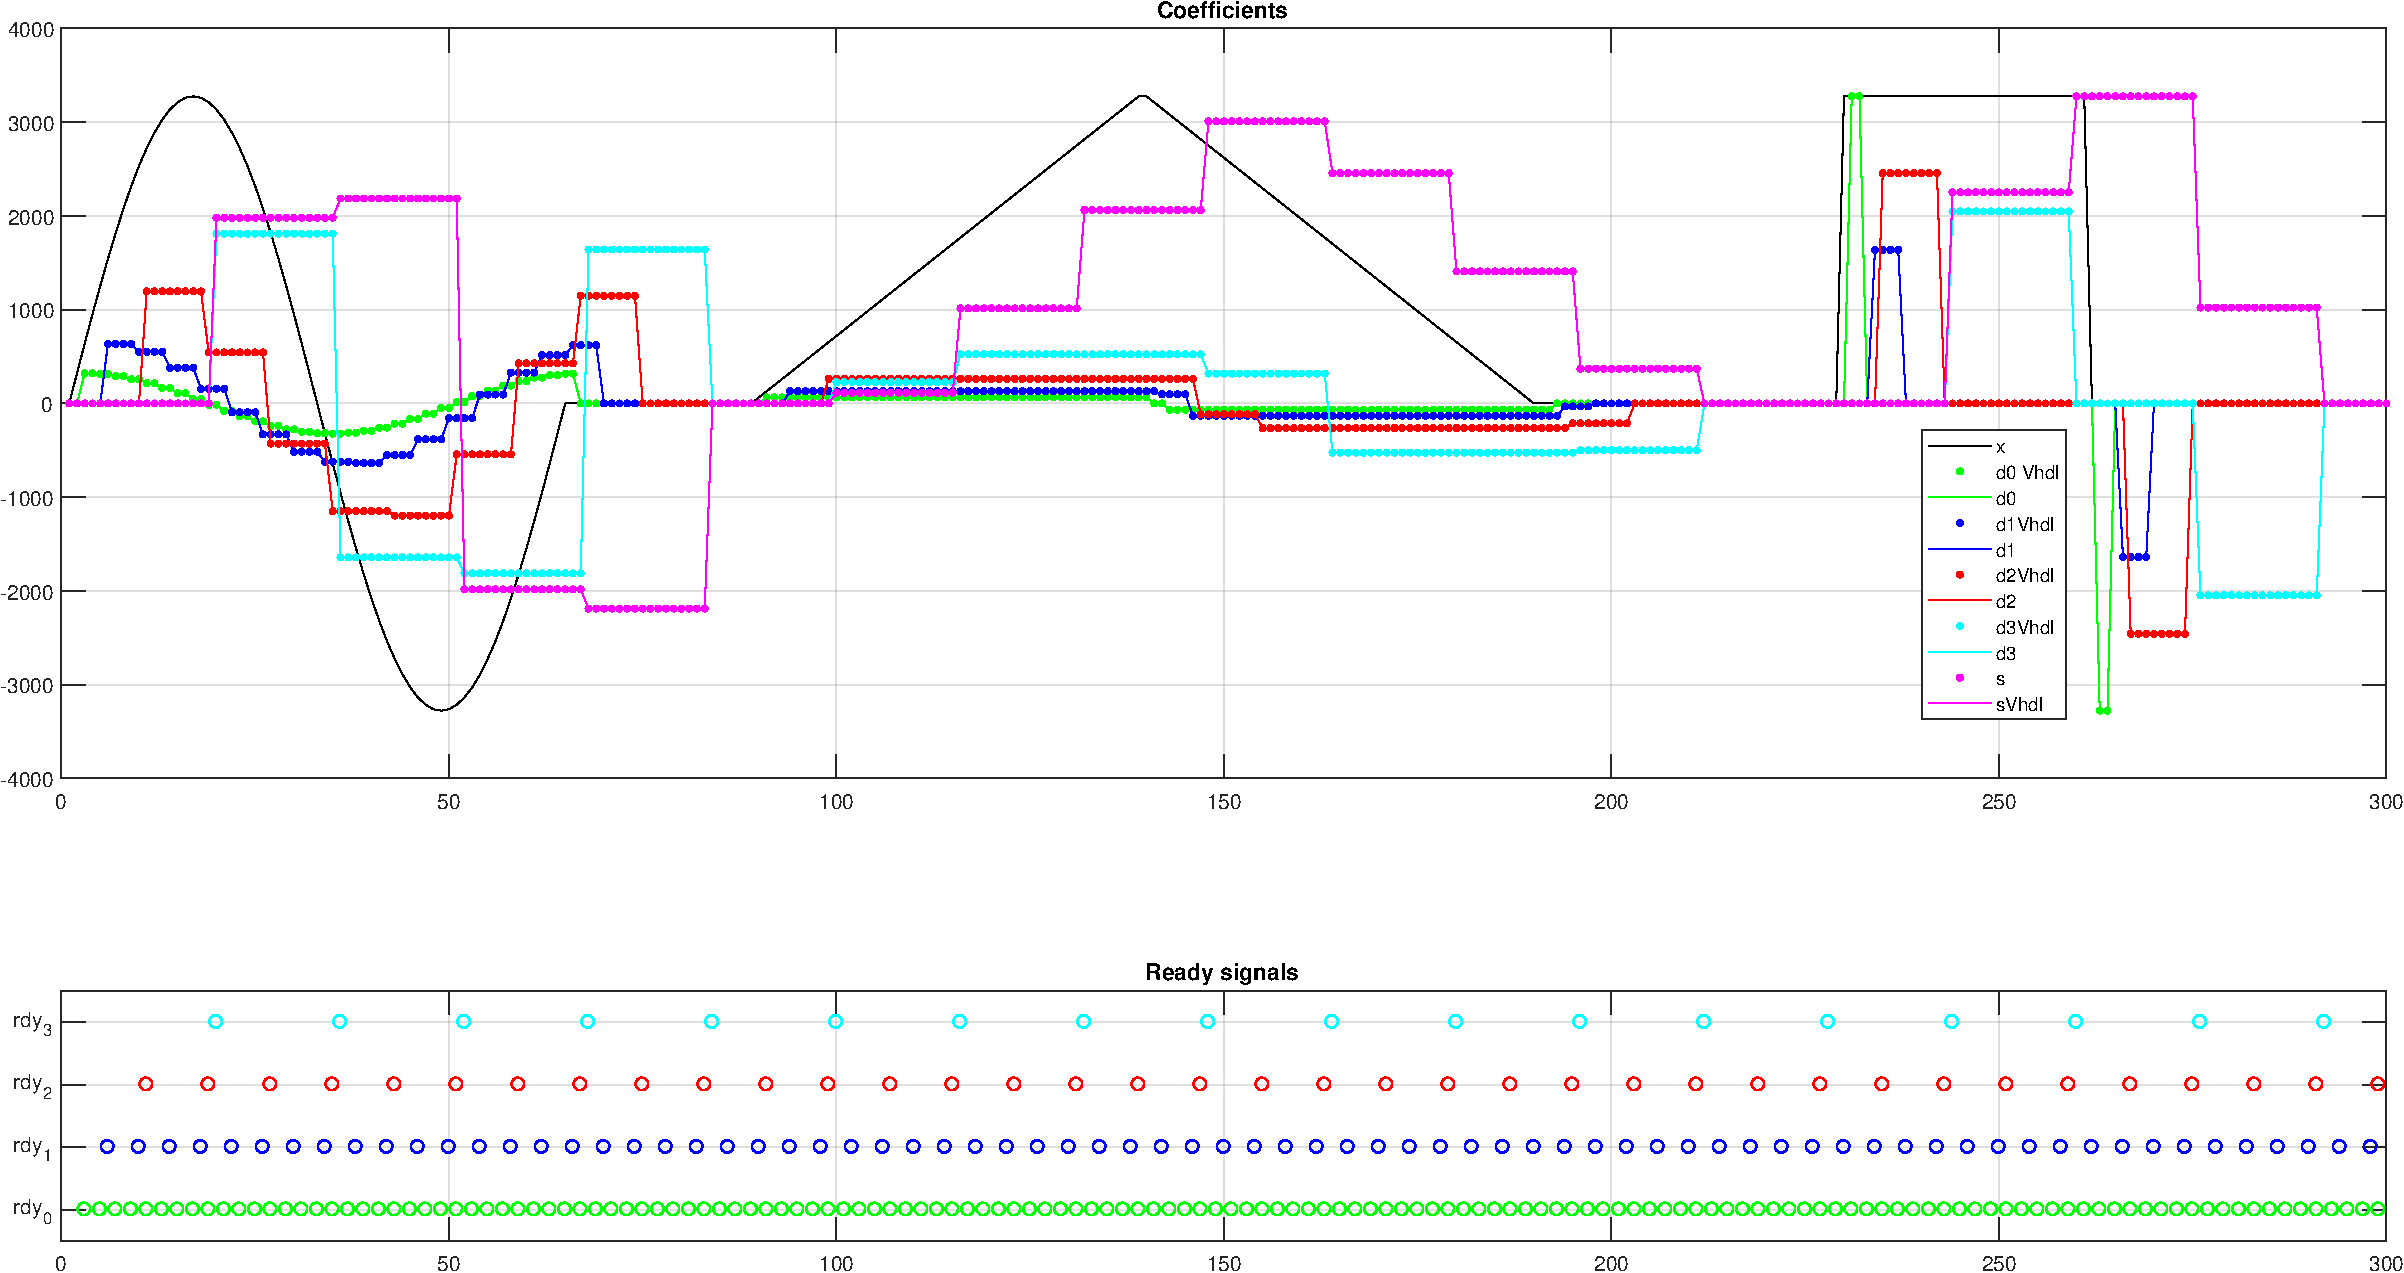
\includegraphics[width=\textwidth]{papers/fpga/images/coefs_with_step.pdf}
	\caption{Coefficients and ready signals after transformation \label{fpga:fig:coeff}}
\end{figure}
The black line is the input signal and the other colors are the different coefficients.
Deeper in the multiresolution analysis, the coefficients are updated more and more infrequently.
The frequency gets halved every step.
Additionally, deeper coefficients are delayed more, as visible in the bottom graph, which shows the ready signals.
The fast changing coefficients correspond to the higher frequencies and the slow changing coefficients correspond to the slower frequencies.

Figure \ref{fpga:fig:coeff_delayed} shows the coefficients and ready signals after delaying as explained in section \ref{fpga:sec:delay}.
\begin{figure}
	\centering
	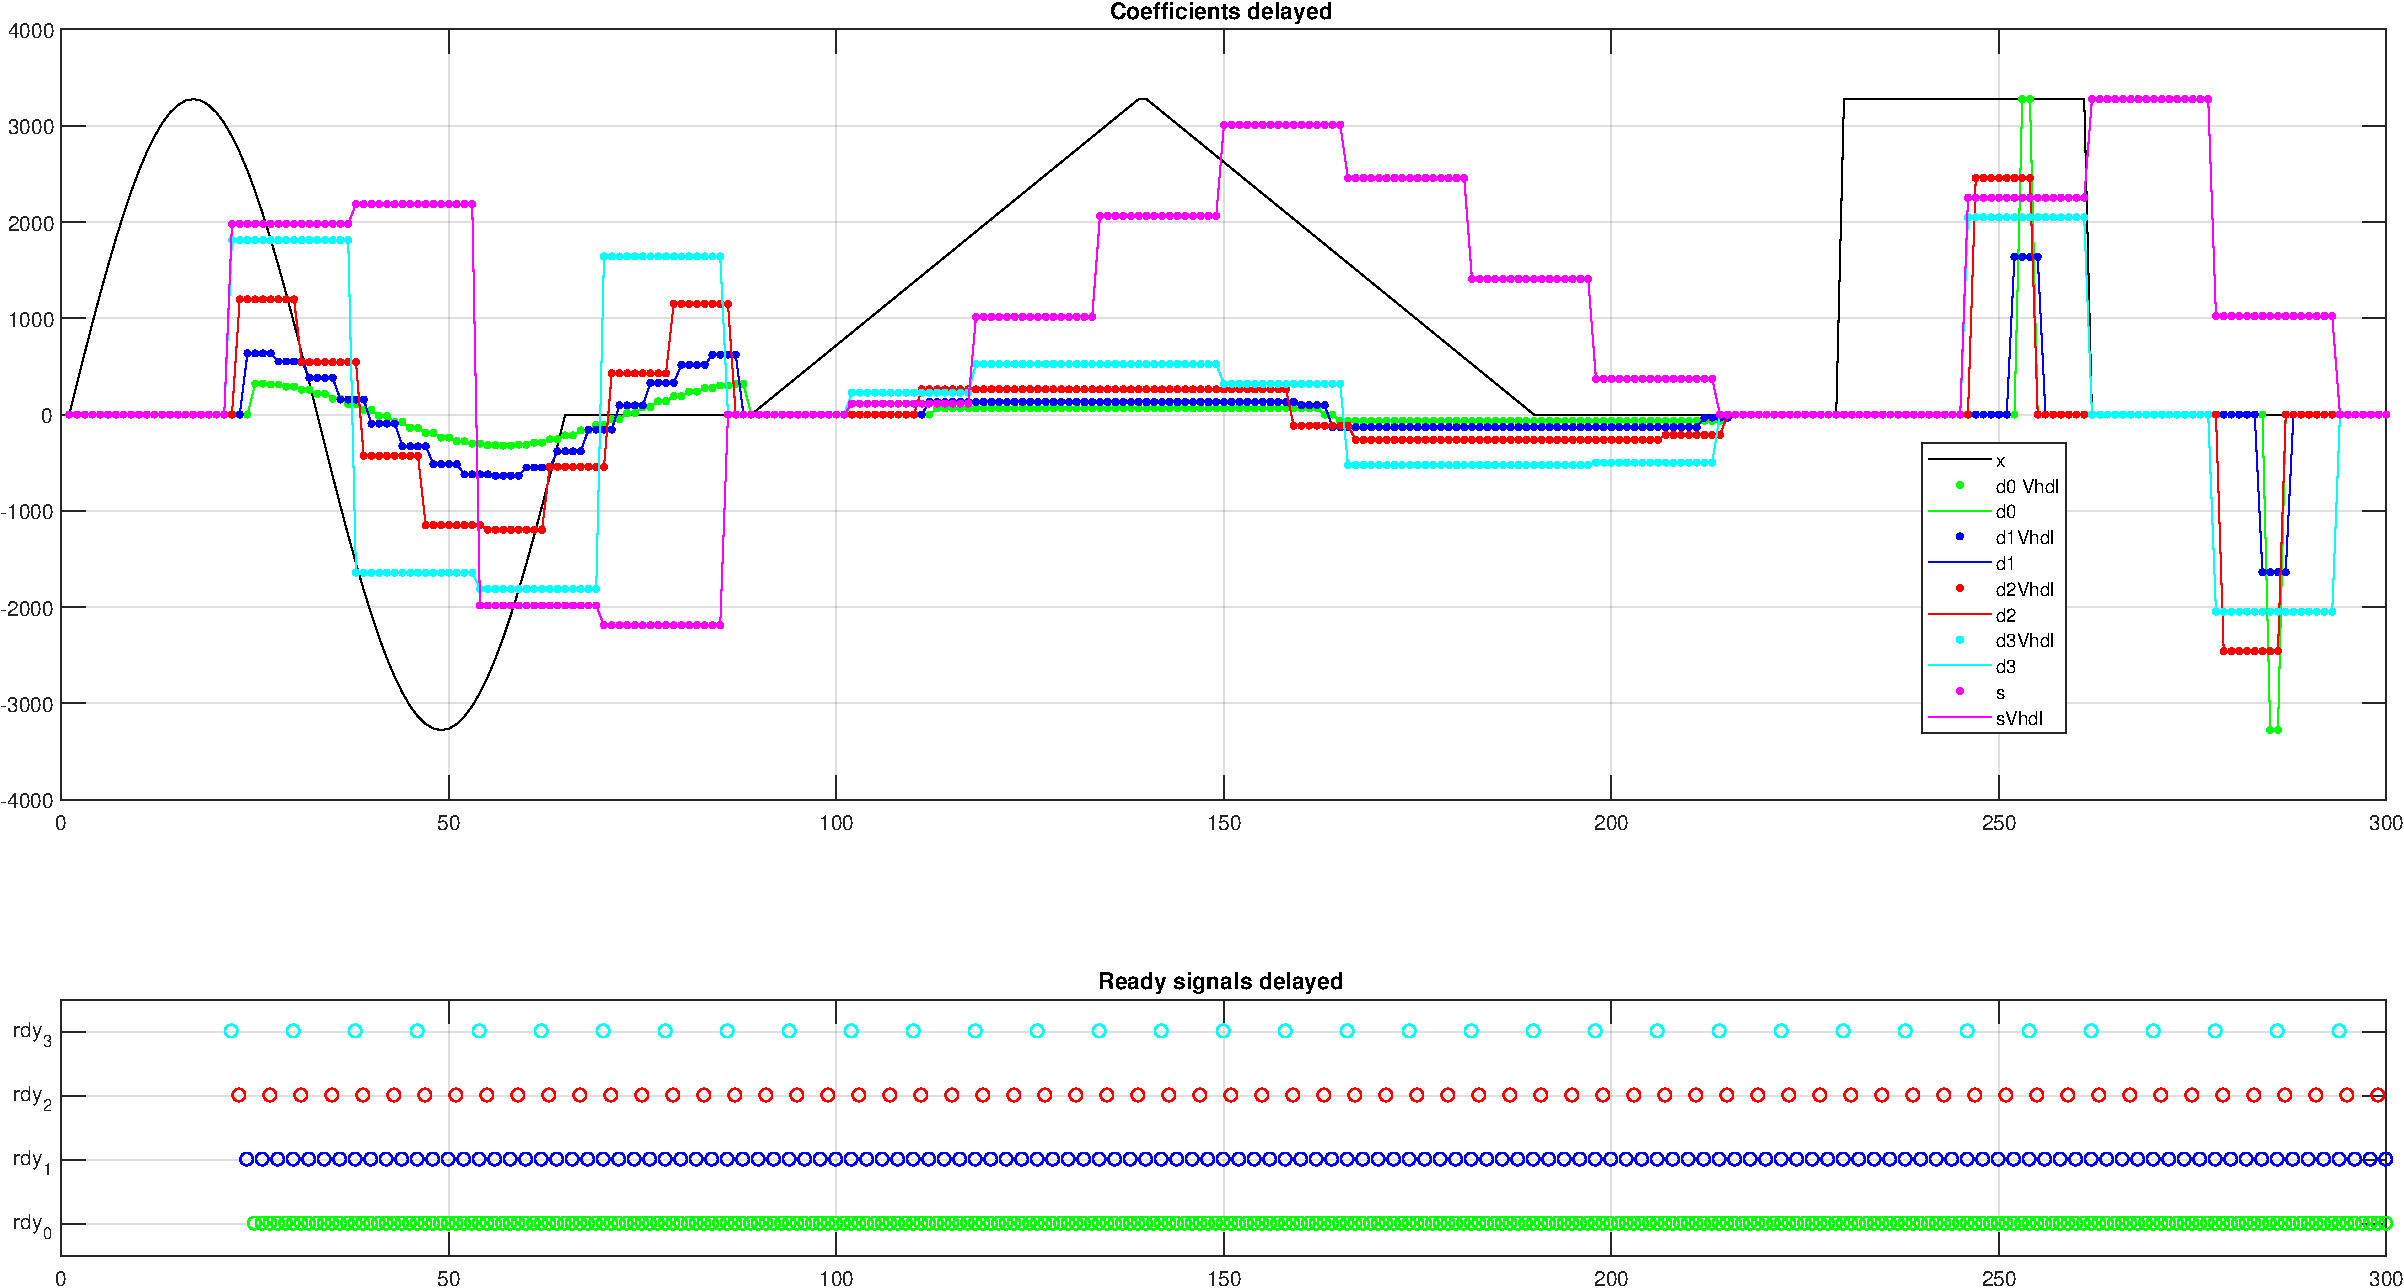
\includegraphics[width=\textwidth]{papers/fpga/images/coefs_delayed_with_step.pdf}
	\caption{Coefficients and ready signals after delaying \label{fpga:fig:coeff_delayed}}
\end{figure}
The coefficients are aligned with a separation of one clock cycle. 
The coefficients for the high frequencies have been delayed more whereas the slow frequencies have been delayed only for a short time. 
In this form, the coefficients can be transformed back to the original signal. 
This is also illustrated in the ready signals.

Figure \ref{fpga:fig:output} shows the final output of the whole pipeline compared to the input signal. 
\begin{figure}
	\centering
	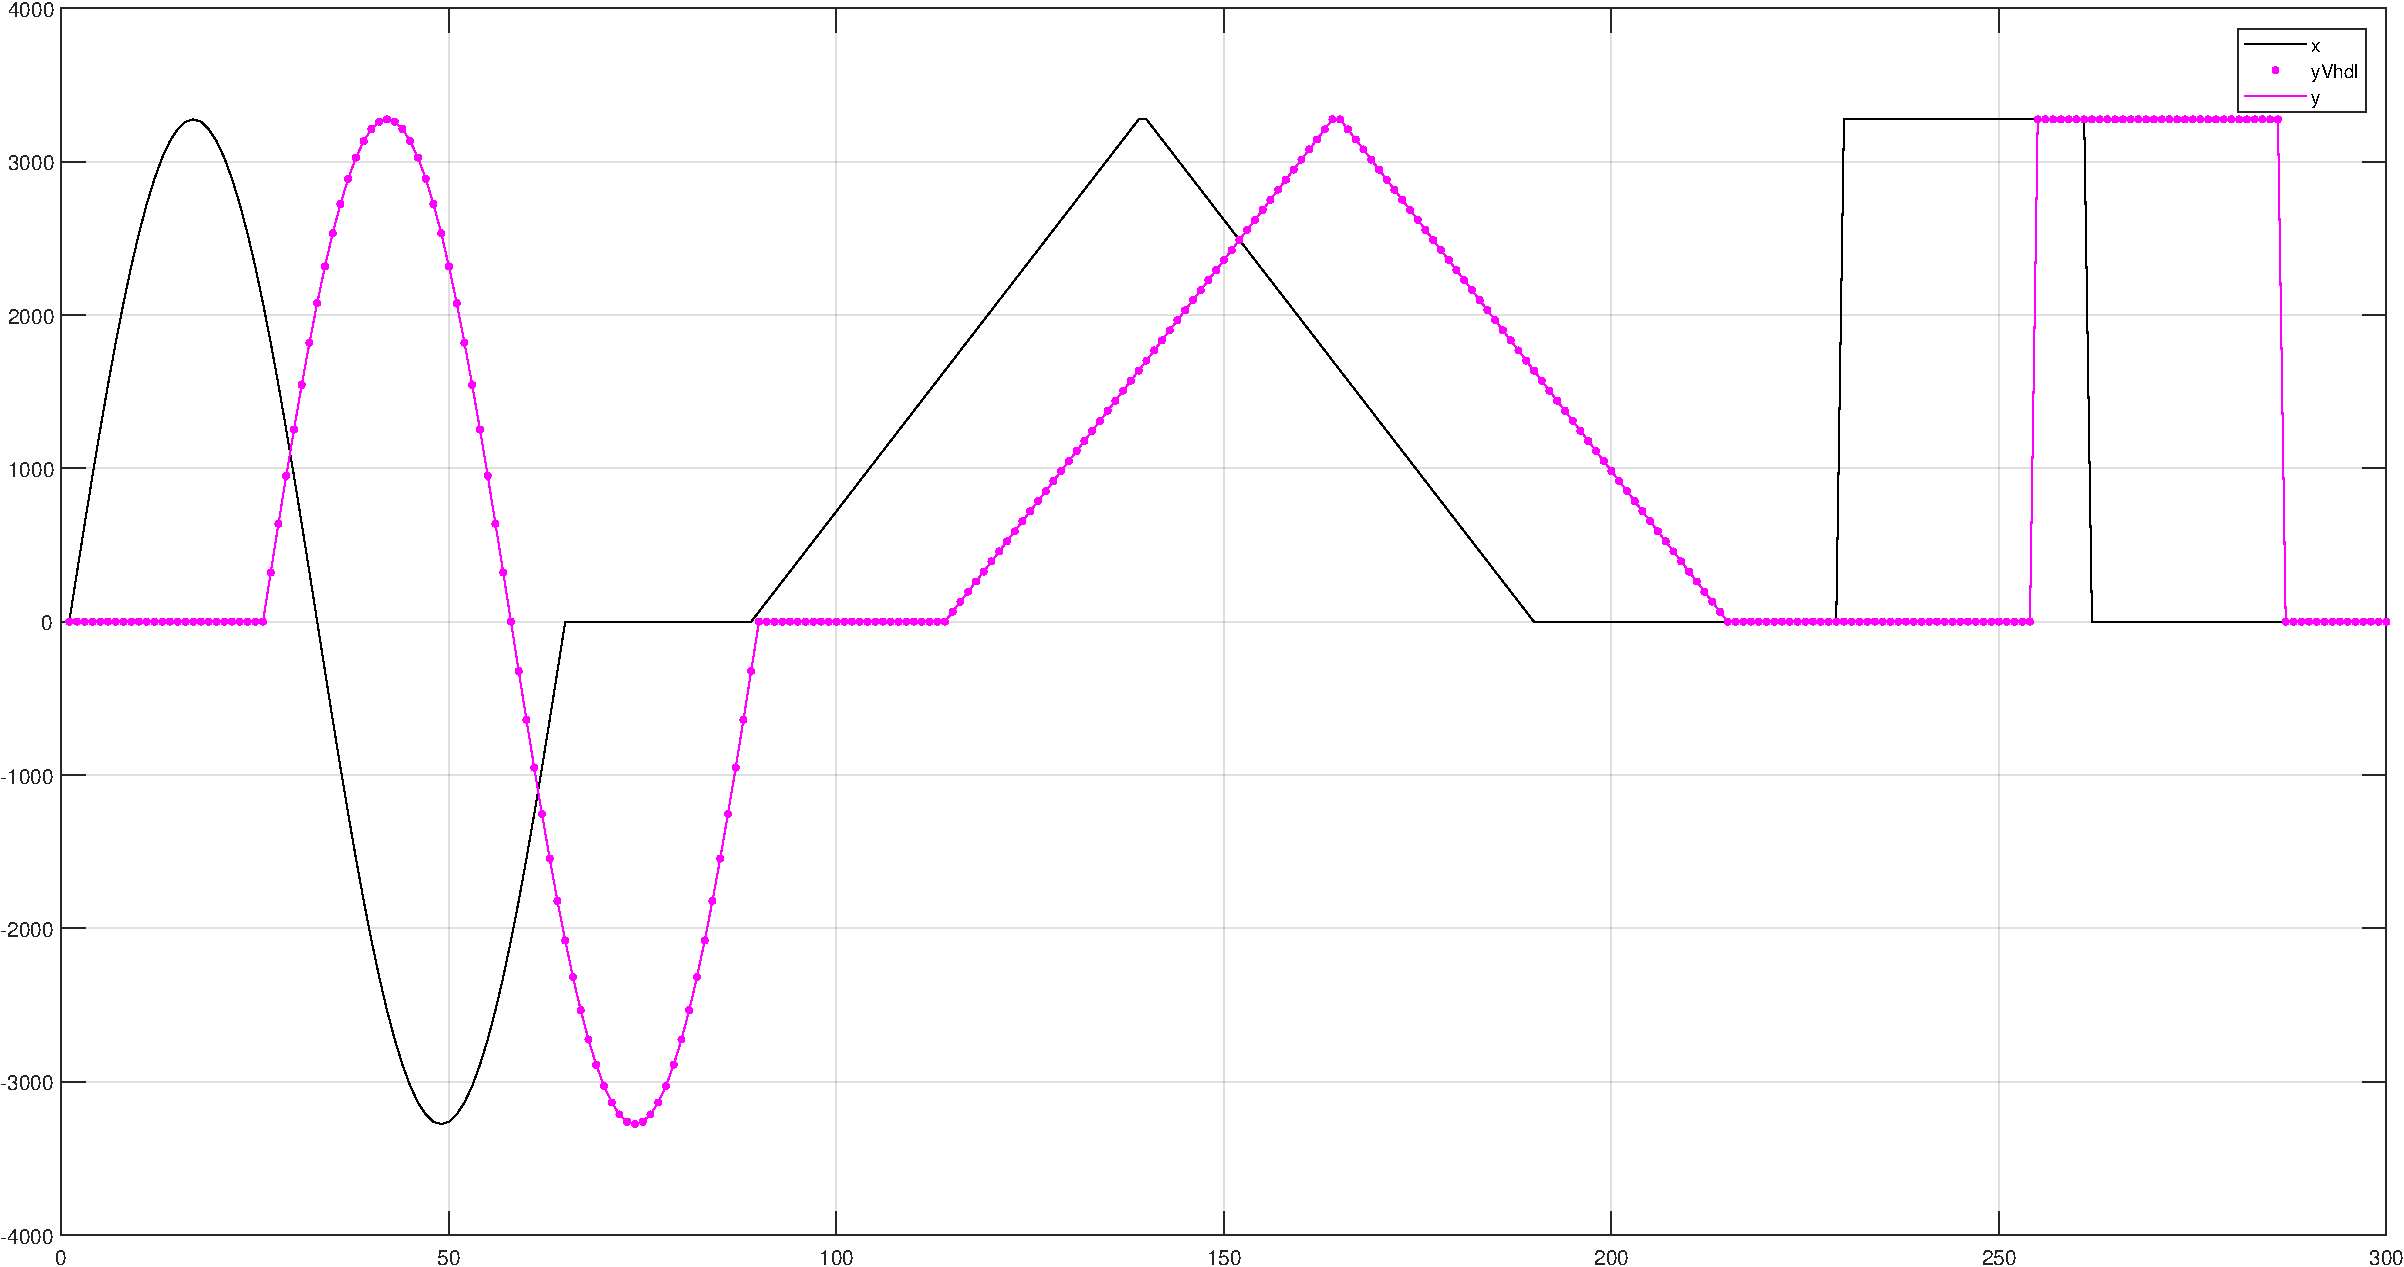
\includegraphics[width=\textwidth]{papers/fpga/images/output_with_step.pdf}
	\caption{Output \label{fpga:fig:output}}
\end{figure}
As expected, the input and output signals are the same when delayed by the processing time of the system.
The pink line is the result of the MATLAB simulation and the pink dots are the results of the Vivado hardware simulation. 

Another interesting insight of the process gives the VHDL simulation graph of Vivado.
Figure \ref{fpga:fig:sim} depicts the signals of the inverse DWT block (\texttt{inv\_branching}).
\begin{figure}
	\centering
	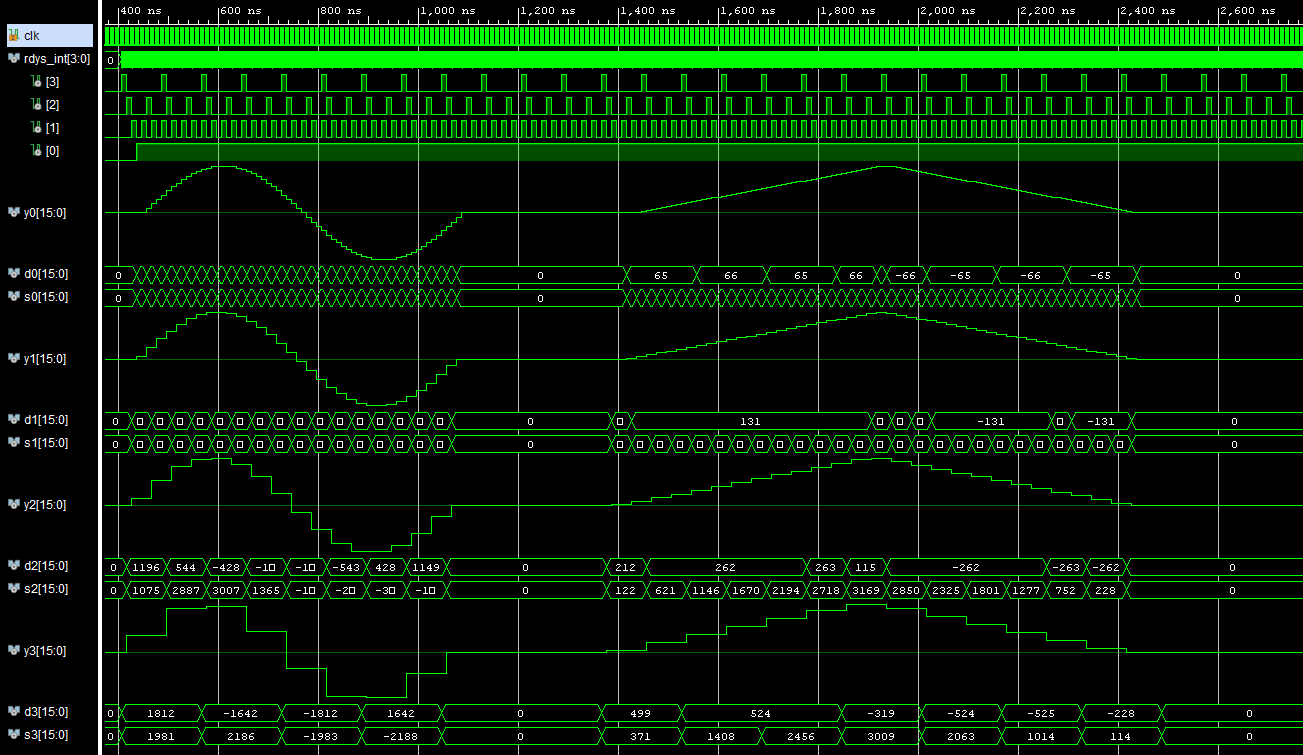
\includegraphics[width=\textwidth]{papers/fpga/images/inv_branching_screenshot.PNG}
	\caption{VHDL simulation view of \texttt{inv\_branching} \label{fpga:fig:sim}}
\end{figure}
The simulation shows the delayed coefficients, as well as the ready signals, as they are reassembled in the inverse DWT (\texttt{inv\_branching}).
The signals are ordered by layers of the multiresolution analysis, where the deepest layer is at the bottom.
As the signal is beeing reconstructed, more and more detail gets added, until the original signal is reconstructed.

\section{Conclusion}
\rhead{Conclusion}

In our view this project was a success.
An efficient algorithm (lifting scheme) for a hardware implementation of the DWT has been found.
Then, a forward and inverse DWT for the Haar wavelet has been implemented in VHDL.
To validate the implementation, a numerical equivalent test bench in MATLAB was built.
Using test benches, we were able to compare our hardware implementation with a working MATLAB simulation.
With the aid of this MATLAB simulation the hardware implementation has been validated and debugged until both versions matched up.

It was satisfying to use some of the knowledge gained in this course and also to add some additional theory to this paper.

The VHDL structure has been implemented in a general structure, which enables the implementation of different, higher order wavelets later. 
The frequency selectivity of the Haar wavelet is low and not suitable for audio applications.
If one would use this implementation on a audio signal, a change of gain of a coefficient would result in various distortions at the output. 
A higher order Daubechies wavelet has increased frequency selectivity, which is more suitable for audio applications.
This way it is possible to boost or attenuate different frequencies in a audio signal with more quality. 

All code of this work is stored in the Github repository belonging to this book \cite{fpga:gitrepo-wavelets}.

\printbibliography[heading=subbibliography]
\end{refsection}
